\documentclass[nofilelist]{cslthse-msc}
% to show a list of used packages at the end of the document, delete the nofilelist option
%\documentclass{cslthse-msc}
\usepackage[utf8]{inputenc}
\usepackage[main=british,swedish]{babel}
\usepackage{amsmath}
%\usepackage{amsfonts}
%%\usepackage{amssymb}
\usepackage{amsthm}
%\usepackage{makeidx}
\usepackage{graphicx}
\usepackage[titletoc, header, page]{appendix}
\usepackage{transparent}
\usepackage{tikz}
\usepackage{enumitem}
\usepackage{listings}
\usetikzlibrary{fit,positioning,shapes.geometric}

\lstdefinestyle{mystyle}{
    basicstyle=\ttfamily,
    breakatwhitespace=false,
    breaklines=true,
    captionpos=b,
    keepspaces=true,
    numbers=left,
    numbersep=5pt,
    showspaces=false,
    showstringspaces=false,
    showtabs=false,
    tabsize=2
}
\lstset{style=mystyle}

% used to display the used files at the end. Select nofilelist as a package option to disable this
\listfiles % initialize

%\geometry{showframe}
%better like this?
\student{Nicholas Boyd Isacsson}{nicholas@isacsson.se}
%\students{Flavius Gruian}{Flavius.Gruian@cs.lth.se}{Camilla Lekebjer}{Camilla.Lekebjer@cs.lth.se}

\thesisnumber{LU-CS-EX: 2023-79} % Magic Number! Do not change unless Birger Swahn asks you to do so!
% default is Master. Uncomment the following for "kandidatarbete"/Bachelor's thesis
%\thesistype{Bachelor}{Kandidatarbete}

%\title{Formatting a Master's Thesis}
\title{Type Checker Generation using Reference Attribute Grammars}
\begin{otherlanguage}{swedish}
\svensktitel{Infoga den Svenska titeln här!}
\end{otherlanguage}

%\onelinetitle
%\twolinestitle
\threelinestitle
%\fourlinestitle

%\subtitle{A {\LaTeX} class}
%\company{The Corporation AB LTD Inc}
%\supervisors{John Deer, \href{mailto:jdeer@company.com}{\texttt{jdeer@company.com}}}{Don Jeer, \href{mailto:djeer@xy.lth.se}{\texttt{djeer@xy.lth.se}}}
\supervisor{Christoph Reichenbach, \href{mailto:christoph.reichenbach@cs.lth.se}{\texttt{christoph.reichenbach@cs.lth.se}}}
%\supervisor{John Deer, \href{mailto:jdeer@company.com}{\texttt{jdeer@company.com}}}
\examiner{Niklas Fors, \href{mailto:niklas.fors@cs.lth.se}{\texttt{niklas.fors@cs.lth.se}}}

\date{\today}
%\date{January 16, 2015}

%\acknowledgements{
%If you want to thank people, do it here, on a separate right-hand page. Both the U.S. \textit{acknowledgments} and the British \textit{acknowledgements} spellings are acceptable.
%
%We would like to thank Lennart Andersson for his feedback on this template.
%
%We would also like thank Camilla Lekebjer for her contribution on this template, as well as Magnus Hultin for his popular science summary class and example document.
%
%Thanks also go to the following (former) students for helping with feedback and suggestions on this template: Mikael Persson, Christoffer Lundgren, Mahmoud Nasser.
%}

\theabstract{
%Your abstract should capture, in English, the whole thesis with focus on the problem and solution in 150 words. It should be placed on a separate right-hand page, with an additional \textit{1cm} margin on both left and right. Avoid acronyms, footnotes, and references in the abstract if possible.
%Leave a \textit{2cm} vertical space after the abstract and provide a few keywords relevant for your report. Use five to six words, of which at most two should be from the title.
}

\keywords{MSc, BSc, template, report, style, structure}

%% Only used to display font sizes
\makeatletter
\newcommand\thefontsize[1]{{#1 \f@size pt\par}}
\makeatother
%%%%%%%%%%

\begin{document}
\renewcommand{\bibname}{References}

\makefrontmatter
\chapter{Introduction} % should give the background of your work. Important parts to cover:
% Give the context of your work, have a short introduction to the area.
While writing software, developers often make mistakes.
Catching these mistakes as early as possible can prevent these bugs from ever reaching production code.
Type checkers are one of the most common static checking methods, ensuring that the correct data types are used, but creating a new type checker is often an arduous process, requiring large amounts of complex code.
Furthermore, making changes to the typing rules of a language can require extensive rewrites in many different parts of the type checker's codebase.
% This can hinder experimentation

In this thesis we examine the feasibility of automating the writing of type checkers, based on the formal definition of the language's typing rules.

% Define the problem you are solving (or trying to solve).
% Specify your contributions. What does this particular work/report bring to the research are or to the body of knowledge? How is the work divided between the co-authors? (This part is essential to pinpoint individual work. For theses with two authors, it is compulsory to identify which author has contributed with which part, both with respect to the work and the report.)
\section{Research questions}
To formulate our goals more concretely, we've set out to answer the following research questions:
\newcommand{\rqone}{What kinds of typing rules can we translate through RAG?}
\newcommand{\rqtwo}{How can we implement the translations and into what form?}
\newcommand{\rqthree}{What are the potential issues of translating typing rules into JastAdd-based RAGs?}
\begin{itemize}
  \item \rqone
  \item \rqtwo
  \item \rqthree
\end{itemize}

\section{Related work} % Maybe move to discussion?
% Describe related work (literature study). Besides listing other work in the area, mention how is it related or relevant to your work. The tradition in some research area is to place this part at the end of the report (check with your supervisor).


\chapter{Background}
%\section{Theory} % should contain the theoretical background needed to understand your work, if necessary.
\section{Type systems}
\subsection{Data types}
\subsection{Type checking}
\subsubsection{Dynamic type checking}
\subsubsection{Static type checking}

\section{Reference Attribute Grammars}
\subsection{Reference Attribute Grammars}
\subsection{JastAdd}
\subsubsection{AST definitions}\label{astdef}


\chapter{Approach/Design} % should contain a description of your solution(s), with all the theoretical background needed. On occasion this is replaced by a subset or all of the following:

\section{Architecture}
In this section we'll be providing an overview of our architecture.
Since it contains many different components, it may be helpful to refer to the overview graph in figure \ref{overviewgraph} while reading.
It represents the flow of the program, with components and artefacts (represented as rectangular boxes) with arrows linking them to actions (elliptical boxes) which in turn have arrows to the new components and artefacts they produce.
The dashed arrows from represent links from the template components that exist in the current experimental state of the project, but in a finished product would instead link to component from the object language's own compilation environment.
%It uses rectangular boxes to represent the concrete data or artefacts of the procedure, and elliptical boxes to represent the actions performed with them.
\begin{figure}[]
  \resizebox{\textwidth}{!}{%
  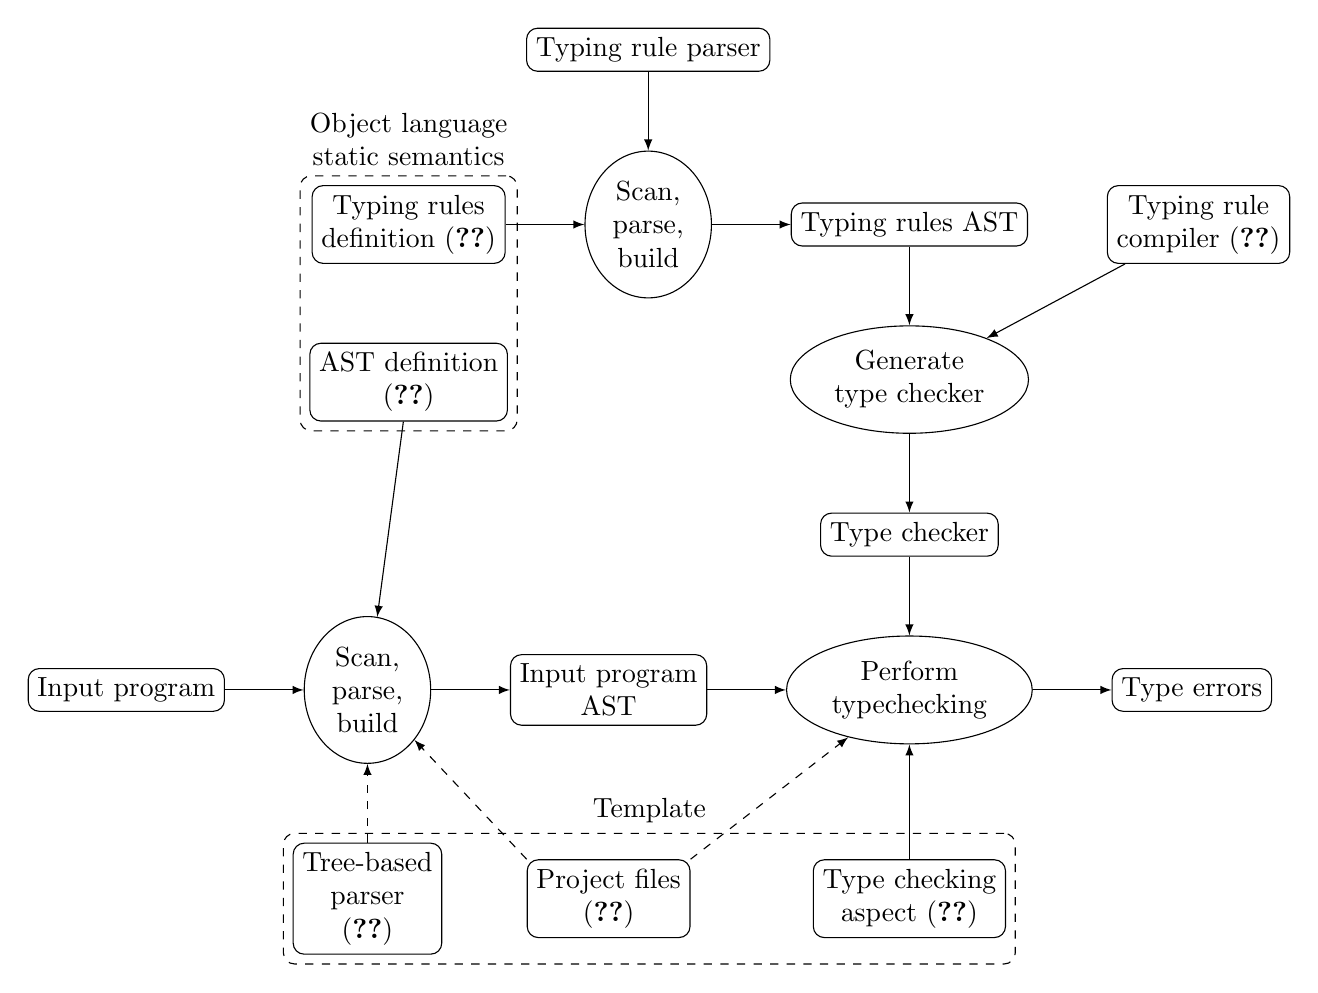
\begin{tikzpicture}[
      every node/.style = {draw=black, rounded corners, align=center},
      every path/.style = {draw, -latex}
    ]
    \node (typerules)                               {Typing rules\\definition (\ref{typingruledefinition})};
    \node (trparsing) [right=of typerules, ellipse] {Scan,\\parse,\\build};
    \node (trparser)  [above=of trparsing]          {Typing rule parser};
    \node (trast)     [right=of trparsing]          {Typing rules AST};

    %\node (typecheckgen) [below=of trast, ellipse, text width=5cm] {
    %  \textbf{Type checker generation}\\
    %  \hrule
    %  \begin{itemize}[noitemsep,topsep=2pt]
    %    \item Copy template
    %    \item Generate type checker from typing rules
    %  \end{itemize}
    %};
    \node (typecheckgen)       [below=of trast, ellipse] {Generate\\type checker};
    \node (typingrulecompiler) [right=of trast]          {Typing rule\\compiler (\ref{typingrulecompiler})};
    \node (typechecker)        [below=of typecheckgen]   {Type checker};

    \node (olast)     [below=of typerules] {AST definition\\(\ref{astdef})};

    \node (outputtypechecking) [below=of typechecker, ellipse] {Perform\\typechecking};
    \node (inputast)           [left=of outputtypechecking]    {Input program\\AST};
    \node (outputparsing)      [left=of inputast, ellipse]     {Scan,\\parse,\\build};
    \node (typeerrors)         [right=of outputtypechecking]   {Type errors};
    \node (inputprog)          [left=of outputparsing]         {Input program};

    %\node (template) [below=of inputast, text width=6cm] {
    %  \textbf{Type checker template}\\
    %  \hrule
    %  \begin{itemize}[noitemsep,topsep=2pt]
    %    \item Scanner, parser, builder
    %    \item Project files
    %    \item Type checking algorithm (\ref{typecheckingalgorithm})
    %  \end{itemize}
    %};
    \node (templateparser)        [below=of outputparsing]                               {Tree-based\\parser\\(\ref{treebasedparser})};
    \node (templateprojectfiles)  at (inputast |- templateparser)                        {Project files\\(\ref{projectfiles})};
    \node (typecheckingalgorithm) at (outputtypechecking |- templateparser)              {Type checking\\aspect (\ref{typecheckingaspect})};
    \node (template)              [dashed, fit=(templateparser) (typecheckingalgorithm)] {};
    \node                         [above, draw=none] at (template.north)                 {Template};

    \node (userinput)   [dashed, fill=none, fit=(typerules) (olast)]                  {};
    \node               [above, draw=none] at (userinput.north)                       {Object language\\static semantics};
    %\node (typechecker) [dashed, fill=none, fit=(outputparsing) (outputtypechecking)] {};
    %\node               [above, draw=none] at (typechecker.north)                     {Type checker};

    \draw (typerules)          to (trparsing);
    \draw (trparser)           to (trparsing);
    \draw (trparsing)          to (trast);
    \draw (trast)              to (typecheckgen);
    \draw (typingrulecompiler) to (typecheckgen);
    \draw (typechecker)        to (outputtypechecking);
    \draw (olast)              to (outputparsing);
    \draw (outputparsing)      to (inputast);
    \draw (inputast)           to (outputtypechecking);
    \draw (outputtypechecking) to (typeerrors);
    \draw (typecheckgen)       to (typechecker);
    \draw (inputprog)          to (outputparsing);

    \draw[dashed] (templateparser)                  to (outputparsing);
    \draw         (typecheckingalgorithm)           to (outputtypechecking);
    \draw[dashed] (templateprojectfiles.north west) to (outputparsing);
    \draw[dashed] (templateprojectfiles.north east) to (outputtypechecking);

  \end{tikzpicture}
  }
  \caption{An overview of the project components and flow.}
  \label{overviewgraph}
\end{figure}

\subsection{Typing rule definition}\label{typingruledefinition}
To express typing rules, we created a simple ASCII representation of the natural deduction notation used by Pierce\cite{Pierce}.
Custom DSL
Include typing rules AST definition (or BNF?)
ASCII representation of natural deduction %BNF (is it BNF?)
\subsubsection{Language}
- Figure of example natural deduction rules (from Pierce?) and ASCII representation
No infix notation
No environments

Our language can express a subset of the notation used by Pierce, with some limitations.
Expressions aren't written in the language's native syntax, instead using a simplified syntax resembling the AST classes.
Values and functions take their names directly from the AST-nodes, and any parameters are included within parenthesis.
This avoids much of the difficulty in parsing different languages, which can have wildly different syntax rules.

Numerical values have not been implemented, but natural numbers can be expressed using Peano numbers\cite{peano}, utilising a zero value and successor function which represents the number incremented by one.
If a language has the syntax \verb|0 + 1| it may instead be represented as \verb|Add(Zero, Succ(Zero))|.


\subsubsection{Parser}
\subsubsection{Abstract syntax tree}

\subsection{Type checker template}
In addition to the compiled files, there are a number of files that are added to the output file that are identical for all generated typecheckers, which we referr to as the template.
Some of these are essential to the functions of the type checker, and others are included for convenience of testing.
We expect that in a real world use case, our software would integrate into an object language's compiler pipeline, and utilise its own parser and project files to provide the abstract syntax tree for our type checking to tie into.
\subsubsection{Parser}\label{treebasedparser}
For testing purposes, our outputted type checker comes with a simple tree-based parser.
Reflection-based parsing

\subsubsection{Project files}\label{projectfiles}
For ease of use the compiler will output a complete runnable Gradle project.
It can parse simplified tree-representations of programs, and utilise these to perform the type checking.

\subsubsection{Type checking aspect}\label{typecheckingaspect}

\subsubsection{Executable}

\subsection{Typing rule compiler}\label{typingrulecompiler}

\subsection{Output type checker}
\subsubsection{Tree-representation}
\subsubsection{Type checking algorithm}\label{typecheckingalgorithm}
Generate code for each node and typing rule
Simple algorithm
Recursive
\subsubsection{Error handling}


%\section{Method (remove this?)} % describe how you go about solving the problem you defined. Also how do you show/prove that your solution actually works, and how well does it work.



\cite{Hedin2011}
\section{Implementation} % if your work involved building an artefact/implementation, give the details here. Note, that this should not, as a rule, be a chronological description of your efforts, but a view of the result. There is a place for insights and lamentation later on in the report, in the Discussion section.
%TODO
\subsection{Type checker generation}
\begin{figure}[h]
\begin{lstlisting}[]
RuleSet ::= Rule*;

abstract Term;
Function : Term ::= <ID> Term*;
Value    : Term ::= <ID>;

Rule ::= <Name> Conclusion:Formula Premises:Formula*;

abstract Formula;
HasType : Formula ::= Expr:Term Ty:TyTerm;

abstract TyTerm;
TyVal   : TyTerm ::= <ID>;
TyVar : TyTerm ::= <ID>;
\end{lstlisting}
  \caption{Typing rules abstract syntax tree specification}
  \label{trastspec}
\end{figure}

The type checker generation is based on a single-responsibility principle, where each node of the abstract syntax tree is responsible for generating the code it corresponds to.
Once typing rules have been parsed, we end up with an abstract syntax tree, in the form of figure \ref{trastspec}, where the \verb|RuleSet| is the root node.
The \verb|RuleSet| node consists of a list of \verb|Rule| nodes, and begins by sorting each rule by which object language node it describes.

The \verb|RuleSet| node then begins by generating the outline of a JastAdd aspect \verb|TypingRules|, and the definition for the method \verb|.type()| for each object language node.
It then calls on the \verb|Rule| node to fill in the implementation of the method.

A \verb|Rule| consists of a name, a conclusion, and a possibly empty list of premises that need to be true for the conclusion to be returned.
In the simplest case of an empty list of premises, the entire content of the rule is generated by the conclusion.
For rules containing premises, the code becomes more involved.
Firstly, any variables or type variables used in the rule need to be declared, followed by a check to ensure each use of a type variable represents a node with the same type.
Then it generates an if-statement corresponding to our premises, by letting each \verb|Premise| generate a boolean expression, all of which get joined by the AND operator.

Both \verb|Premise|s and \verb|Conclusion|s are represented by the same abstract class \verb|Formula|, which currently contains a single implementation \verb|HasType|, consisting of an expression and a type.
Depending on whether it is used as a premise or conclusion, it can either represent that the expression must have the specified type or that the expression should be given the specified type.

\subsection{Type checker design}
The provided typing rules compile into \verb|type()| methods, which return a value from the Type interface.
For the most simple typing rules, this method's implementation will consist of a single return statement.

Types are declared in an AST specification, currently provided by the template, allowing simple type hierarchies.


\chapter{Evaluation} % is the part where you present the finds. Depending on the area this part contains a subset or all of the following:
%\section{Experimental Setup} % should describe the details of the method used to evaluate your solution(s)/approach. Sometimes this is already addressed in the \textbf{Method}, sometimes this part replaces \textbf{Method}.
\section{Results} % contains the data (as tables, graphs) obtained via experiments  (benchmarking, polls, interviews). Here you should also describe the individual tables or graphs in text, pointing out interesting outliers and trends.
%\subsection{Input/output examples, with descriptions}
\subsection{Bools}

\begin{figure}[h]
\begin{lstlisting}[]
Expression ::= Term;

abstract Term;
True  : Term;
False : Term;
Or    : Term ::= Left:Term Right:Term;
Zero  : Term;
\end{lstlisting}
  \caption{AST specification for the Bools language}
  \label{boolsast}
\end{figure}
\begin{figure}[h]
\begin{lstlisting}[]
[T-True]
-----------
True : Bool

[T-False]
------------
False : Bool

[T-Or]
left : Bool,
right : Bool
----------------------
Or(left, right) : Bool

[T-Zero]
----------
Zero : Int
\end{lstlisting}
  \caption{Typing rules for the Bools language}
  \label{boolstr}
\end{figure}

\begin{figure}[h]
\begin{lstlisting}[]
aspect TypingRules {

syn Type Zero.type() {
return new Int();}
syn Type Or.type() {
ASTNode left = getChild(0);
ASTNode right = getChild(1);

if(left.type().matches(new Bool()) && right.type().matches(new Bool())) {
return new Bool();
}
throw new RuntimeException("Typechecking failed");
}
syn Type True.type() {
return new Bool();}
syn Type False.type() {
return new Bool();}
}
\end{lstlisting}
  \caption{Generated typing rules for the Bools language}
  \label{boolstrgen}
\end{figure}
A simple example of a language is provided in figure \ref{boolsast}, consisting of three values, \verb|True|, \verb|False| and \verb|Zero|; and the boolean operator \verb|Or| with two parameters, Left and Right.
In the AST specification, there are no limitations on what terms can be provided as parameters to the \verb|Or| operator, allowing illogical constructs such as \verb|Or(True, Zero)|.

To prevent cases like these, we define typing rules via the specification in figure \ref{boolstr}.
The typing rules for \verb|True|, \verb|False| and \verb|Zero| contain no premises and define the type as \verb|Bool| and \verb|Int| as appropriate.
The typing rule for the \verb|Or| operator, which takes two parameters \verb|left| and \verb|right|, contains two premises, specifying that the \verb|Or| operator has the type \verb|Bool| only if both the \verb|left| and \verb|right| terms also have the type \verb|Bool|.

The typing rules from figure \ref{boolstr} generate the type definitions in \ref{boolstrgen}.
The simple rule definitions for the values compile into equally simple implementations, consisting of a single return statement of a newly constructed \verb|Type| object.
For the \verb|Or| node, the code becomes slightly more complex.
First two variables are defined, corresponding to the parameters in the typing rule, and assigned to the children with the index corresponding to the position among the parameters.
This is followed by an if-statement, recusively evaluating the children's types and comparing the result the type demanded in the premise.
If the condition is true, a \verb|Bool| type is returned.
If not, a runtime exception is thrown to convey a type error.

\subsection{If-else extension}

\begin{figure}[h]
\begin{lstlisting}[]
IfElse : Term ::= Cond:Term Then:Term Else:Term;
\end{lstlisting}
  \caption{Extension for the Bools AST}
  \label{ifelseast}
\end{figure}
\begin{figure}[h]
\begin{lstlisting}[]
[T-IfElse]
x: Bool,
y: a,
z: a
------------------
IfElse(x, y, z): a
\end{lstlisting}
  \caption{Extension for the Bools typing rules with an if-else term}
  \label{ifelsetr}
\end{figure}
\begin{figure}[h]
\begin{lstlisting}[]
syn Type IfElse.type() {
ASTNode x = getChild(0);
ASTNode y = getChild(1);
ASTNode z = getChild(2);

Type tyvar_a = null;
if(tyvar_a == null) tyvar_a = y.type();
else if (!tyvar_a.matches(y.type()))
throw new RuntimeException("Typechecking failed: Type variable mismatch");
if(tyvar_a == null) tyvar_a = z.type();
else if (!tyvar_a.matches(z.type()))
throw new RuntimeException("Typechecking failed: Type variable mismatch");
if(x.type().matches(new Bool()) && y.type().matches(tyvar_a) && z.type().matches(tyvar_a)) {
return tyvar_a;
}
throw new RuntimeException("Typechecking failed");
}
\end{lstlisting}
  \caption{Generated typing rules for the if-else term}
  \label{boolstrgen}
\end{figure}

%\begin{figure}
%\centering
%  \begin{minipage}[b]{.4\textwidth}
%  \centering
%\begin{lstlisting}[]
%[T-IfElse]
%x: Bool,
%y: a,
%z: a
%---------
%IfElse(x, y, z): a
%\end{lstlisting}
%  \captionof{figure}{A figure}
%  \label{fig:test1}
%\end{minipage}%
%\begin{minipage}[b]{.6\textwidth}
%  \centering
%\begin{lstlisting}[]
%syn Type IfElse.type() {
%ASTNode x = getChild(0);
%ASTNode y = getChild(1);
%ASTNode z = getChild(2);
%
%Type tyvar_a = null;
%if(tyvar_a == null) tyvar_a = y.type();
%else if (!tyvar_a.matches(y.type()))
%throw new RuntimeException("Typechecking failed: Type variable mismatch");
%if(tyvar_a == null) tyvar_a = z.type();
%else if (!tyvar_a.matches(z.type()))
%throw new RuntimeException("Typechecking failed: Type variable mismatch");
%if(x.type().matches(new Bool()) && y.type().matches(tyvar_a) && z.type().matches(tyvar_a)) {
%return tyvar_a;
%}
%throw new RuntimeException("Typechecking failed");
%}
%\end{lstlisting}
%  \captionof{figure}{Another figure}
%  \label{fig:test2}
%\end{minipage}
%\end{figure}
Extend bool with if-statement to show type variables
\section{Research questions}
\subsection{\rqone}

\subsection{\rqtwo}
\subsection{\rqthree}
%Splitting code between multiple JastAdd components (and java) can get messy
Writing idiomatic JastAdd components often requires splitting your code into many different places.
We attempted to keep each node in the tree responsible for generating the code it corresponds to, which avoids parent nodes having to check their children's structure with \verb|isInstanceOf|, but also means even generating a simple rule can require a dozen calls between different nodes.
There's a tradeoff to be made between the single responsibility of each component making it easy to verify its correctness, but the complicated interdependence making it hard to grasp the full picture.

Using JastAdd simultaneously as a library and a build component

%Having to use a hacky method to access private JastAdd methods to parse a second AST at runtime. (Beyond jastadd's scope?)
Some of the features we intended to support, such as verifying that typing rules correspond to valid nodes within the object language AST, were complicated by having to parse the object language AST at runtime, using JastAdd as a library rather than a build tool.
JastAdd does not expose any methods for parsing an AST tree at runtime, and we had to access undocumented, private methods through Java's reflection API to get the relevant information.
Unfortunately, the resulting data was hard to work with and we could not allocate enough time to implement the planned features.
It may be that this use case is beyond the intended scope of JastAdd, or it is perhaps only poorly documented.
In either case, while our experimentation has shown it to be technically possible, the complexity is worth bearing in mind for future work.


\chapter{Discussion} % allows for a longer discussion and interpretation of the results from the evaluation, including extrapolations and/or expected impact. Focus here on a broader view of the results, talking about the relation between the different finds.\footnote{Bad practice is to display graphs in Results and then describe them textually one by one in here. No! Both sections should have some discussion, but one targets individual finds and the other tries to bridge between these adopting a more overarching viewpoint.} This might also be a good place to describe your positive and negative experiences related to the work you carried out.
% Occasionally these sections are intermingled, if this allows for a better presentation of your work. However, try to distinguish between measurements or hard data (results) and extrapolations, interpretations, or speculations (discussion).
\section{Supported features}
\section{Development learnings}

\chapter{Conclusions} % should summarize your findings and possible improvements or recommendations.
\section{Summary of findings}
\section{Future work}
Improved error handling
Check for completeness of rules
Verify rules against AST
Handle multiple rules for the same node (add(int, int): int, add(double, double): double)
Better support for numbers, strings, etc.


% Should use consistent formatting when it comes to Names ("FirstName LastName", or "F. LastName")
%\printbibliography
\makebibliography{MyMSc} % is a must in a scientific report. {\LaTeX} and \texttt{bibtex} offer great support for  handling references and automatically generating bibliographies.

\begin{appendices} %should contain lengthy details of the experimental setup, mathematical proofs, code download information, and shorter code snippets. Avoid longer code listings. Source code should rather be made available for download on a website or on-line repository of your choosing.
Git repository link

% display used packages information unless noflielist is used in the cslthse-msc package option
\printfilelist

%make sure we're on even page with the pop-sci
\checkoddpage
\ifoddpage
\else
   \newpage
   \thispagestyle{empty}
   \mbox{ }
\fi
\includepdf[pages={1}]{popsci/popsci.pdf}
\end{appendices}

\end{document}
